% !TEX root = ../master-thesis.tex



\textbf{Classical Monte Carlo.} To accurately model the classical trajectories of atoms undergoing matter-wave magnification, a numerical Monte Carlo approach combined with the fourth-order Runge-Kutta (RK4) integration method is employed. The RK4 method numerically solves ordinary differential equations with high accuracy, making it ideal for simulating classical dynamics governed by Newtonian mechanics.

% In our simulations, several physically relevant potentials appear regularly:
% \begin{equation}
% V_\text{harm}(r) = \frac{1}{2} m \omega^2 r^2,
% \hspace{5 mm} 
% V_\text{gauss}(r) = V_0 \exp\left(-\frac{r^2}{2w^2}\right),
% \hspace{5 mm} 
% V_\text{lorentz}(r) = \frac{V_0}{1 + (\frac{1}{4} r^2 / w^2)}.
% \end{equation}
% with the trapping frequency $\omega$, the radial distance $r$ from the trap center, the potential depth $V_0$, and the Gaussian beam waist $w$.


The particle trajectories are determined by solving Newton's equations of motion:
\begin{equation}
m \frac{d^2 \vc{r}}{dt^2} = -\nabla V(\vc{r}),
\end{equation}
where $m$ is the particle mass, and $V(\vc{r})$ denotes the potential acting on the atoms. 
The RK4 algorithm explicitly updates positions and momenta at each timestep $\Delta t$ as follows. Consider a state vector $\vc{y}(t) = (\vc{r}(t), \vc{p}(t))$. Time evolution is determined by:
\begin{equation*}
\frac{d \vc{y}(t)}{dt} = \vc{f}(t,\ \vc{y}(t)),
\hspace{5 mm} 
\vc{f}(t, \vc{y}(t)) = \left(\frac{\vc{p}(t)}{m}, -\nabla V(\vc{r}(t))\right).
\end{equation*}
where the right-hand side vector $\vc{f}(t, \vc{y}(t))$ encapsulates both position and momentum updates. 

The RK4 integration method proceeds through intermediate stages:
\begin{align*}
\vc{k}_1 &= \vc{f}(t,\ \vc{y}(t)), \\
\vc{k}_2 &= \vc{f}\left(t + \tfrac{1}{2}\Delta t,\ \vc{y}(t) + \tfrac{1}{2}\vc{k}_1\right), \\
\vc{k}_3 &= \vc{f}\left(t + \tfrac{1}{2}\Delta t,\ \vc{y}(t) + \tfrac{1}{2}\vc{k}_2\right), \\
\vc{k}_4 &= \vc{f}\left(t + \Delta t,\ \vc{y}(t) + \vc{k}_3\right),
\end{align*}
resulting in the updated state vector:
\begin{equation*}
\vc{y}(t + \Delta t) = \vc{y}(t) + \tfrac{\Delta t}{6}\left(\vc{k}_1 + 2\vc{k}_2 + 2\vc{k}_3 + \vc{k}_4\right).
\end{equation*}

Initial conditions in Monte Carlo simulations are sampled according to experimentally realistic normal distributions relevant for trapped atoms. The trajectories evolve numerically via the RK4 method with sufficiently small timesteps to ensure numerical precision and stability. GPU acceleration significantly enhances computational performance, allowing the simulation of approximately $1.6 \times 10^6$ particles for 1000 RK4 steps in approximately 4 seconds (benchmarking performed on an NVIDIA A100 GPU). In contrast, the same computation performed on a standard CPU (Intel Xeon Gold 6330) typically requires about 100 seconds, highlighting the significant speedup provided by GPU implementation. 
% This computational efficiency enables extensive exploration of parameter spaces and detailed characterization of magnified atomic distributions, directly supporting the simulation results presented throughout this thesis.

The subsequent section describes our quantum mechanical simulations employing the split-step method, which complement the classical approach and address quantum-statistical effectsfor fermionic atoms.



\begin{figure}
    \centering
    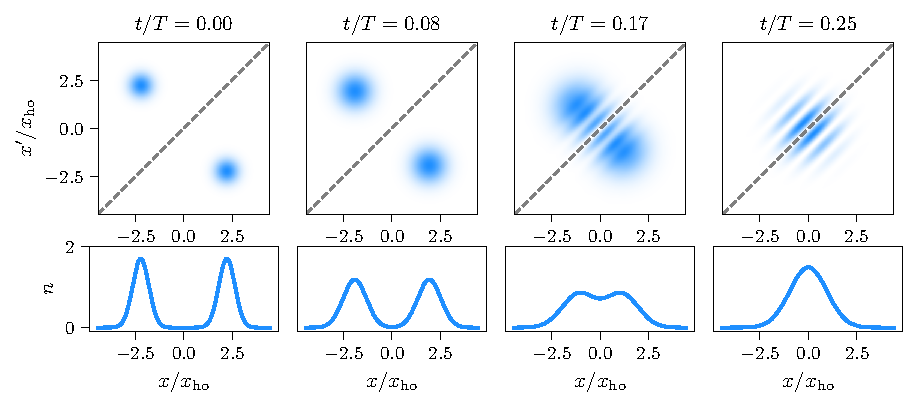
\includegraphics{fig-py/interference.pdf}
    \caption{
        \textbf{Two-fermion dynamics in a 1D harmonic trap: quantum statistics.}
        Top row: Time evolution of the two-particle correlation function $P_2(x,x')$ for two fermions in a harmonic potential. The characteristic anti-bunching dip along the diagonal reflects fermionic quantum statistics, contrasting the bunching peak expected for bosons. Bottom row: Corresponding single-particle density profiles $n(x)$, which remain indistinguishable from the bosonic case, highlighting the necessity of two-particle correlations to probe quantum statistics.
        }
    \label{fig:interference}
\end{figure}



\textbf{Split-step method.}
Complementing the classical Monte Carlo approach, in this work quantum mechanical simulations were employed to capture wavefunction dynamics during matter-wave magnification. Specifically, we utilize the split-step Fourier method, which efficiently solves the time-dependent Schrödinger equation, particularly suitable for systems with spatially varying potentials and wavefunction evolution.

The evolution of the atomic wavefunction $\psi(\vc{r}, t)$ is governed by the time-dependent Schrödinger equation:
\begin{equation*}
i\hbar\frac{\partial}{\partial t}\psi(\vc{r}, t) = \left(-\frac{\hbar^2}{2m}\nabla^2 + V(\vc{r})\right)\psi(\vc{r}, t).
\end{equation*}
The split-step method leverages the separation of kinetic and potential energy terms. The propagation over a timestep $\Delta t$ can be approximated by splitting the evolution operator into kinetic and potential contributions:
\begin{equation*}
\psi(\vc{r}, t + \Delta t) \approx e^{-i\frac{\Delta t}{2\hbar}V(\vc{r})} e^{-i\frac{\Delta t}{\hbar}\frac{\hat{p}^2}{2m}} e^{-i\frac{\Delta t}{2\hbar}V(\vc{r})}\psi(\vc{r}, t).
\end{equation*}

The kinetic operator is naturally handled in momentum space via the Fourier transform, as it becomes diagonal:
\begin{equation*}
\exp\left(-i\frac{\Delta t}{\hbar}\frac{\hat{p}^2}{2m}\right)\psi(\vc{r}, t) = \mathcal{F}^{-1}\left[\exp\left(-i\frac{\Delta t}{\hbar}\frac{\hbar^2 k^2}{2m}\right)\mathcal{F}{\psi(\vc{r}, t)}\right],
\end{equation*}
where $\mathcal{F}$ denotes the Fourier transform, and $k$ is the momentum-space coordinate. Thus, each evolution step avoids the stringent Courant–Friedrichs–Lewy (CFL) condition encountered in purely spatial methods, allowing for larger and more efficient timesteps.

Quantum treatment via the split-step method becomes particularly relevant when analyzing phenomena sensitive to quantum statistics. While average densities for ensembles of non-interacting atoms can be accurately captured using classical descriptions, quantum approaches are indispensable when studying relative positions of particles within individual realizations—especially for fermions. This is illustrated by considering two fermions in a harmonic trap, where quantum statistics significantly influence the spatial correlation patterns, producing characteristic anti-bunching behavior distinctly observable in the two-particle correlation function $P_2(x,x')$ \cite{bergschneider_experimental_2019}.

Specifically, the fermionic nature imposes Pauli exclusion, manifesting as a pronounced dip in $P_2(x,x')$ along the line $x=x'$, contrasting sharply with the bunching observed in bosonic systems. Such quantum-statistical features, shown explicitly in Fig.~\ref{fig:interference}, are not captured by classical simulations and underscore the necessity of quantum modeling methods like the split-step Fourier approach. Consequently, this technique complements the classical Monte Carlo simulations, providing a numerical framework to support the experimental realization of matter-wave magnification schemes described throughout this work.

The next subsection discusses in detail the Voronoi diagram-based method introduced to adaptively define regions of interest (ROI), mitigating spatial distortions inherent in the magnified atomic distributions.


\textbf{ROI with Voronoi diagrams.}
While matter-wave magnification significantly improves the spatial resolution for atomic imaging, practical implementations face challenges arising from anharmonicities and other distortions inherent in realistic trapping potentials. These distortions can lead to irregular spatial distributions, complicating reliable single-atom detection. Consequently, defining appropriate regions of interest (ROI) for each magnified atomic pattern becomes essential to ensure high detection fidelity.

In this work, a robust solution was introduced by employing Voronoi diagrams to adapt the ROI according to the actual spatial distributions observed after magnification. Voronoi diagrams partition a plane into distinct regions based on the distance to a specified set of points, known as "seeds". Each region contains exactly one seed, and any given point within a region is closer to its corresponding seed than to any other seed. Formally, for a set of seed points $\{\mathbf{s}_i\}$, the Voronoi region $R_i$ associated with seed $\mathbf{s}_i$ is defined as:
\begin{equation}
R\_i = {\mathbf{r} \mid |\mathbf{r}-\mathbf{s}\_i| \leq |\mathbf{r}-\mathbf{s}\_j|, \hspace{5 mm} \forall j \neq i}.
\end{equation}

By using the experimentally determined average final atom positions after the magnification process as seeds, Voronoi diagrams naturally provide adaptive ROIs tailored to distorted atom distributions. This ensures each ROI captures the atom signal associated with its corresponding trap site, even under anharmonic distortion. Voronoi-based ROI allocation minimizes signal contamination between neighboring sites, as each ROI is constructed explicitly to maximize separation from adjacent seed points, thereby reducing overlap.

Within the scope of this thesis, Voronoi diagram-based ROI adaptation was proposed and validated as a method for improving atom detection reliability after MWM. As demonstrated in Fig.~\ref{fig:mwm}b, applying Voronoi diagrams enhances detection by systematically accounting for magnification-induced distortions in atomic distributions. 


\textbf{Summary}. In this subsection, the concept of matter-wave magnification (MWM) was introduced, a powerful approach to enhance spatial resolution in quantum gas microscopy beyond conventional optical limitations.
To accurately describe and optimize the MWM process, two numerical methodologies were implemented. The classical Monte Carlo approach with fourth-order Runge-Kutta (RK4) integration provides efficient simulation of large ensembles of atoms, effectively capturing macroscopic ensemble dynamics. In parallel, the split-step Fourier method addresses quantum-mechanical wavefunction evolution, essential when quantum-statistical effects such as fermionic anti-bunching become relevant. Distortions induced by potential anharmonicities were addressed using Voronoi diagrams. This adaptive method adjusts regions of interest based on observed atomic distributions, ensuring robust atom detection even under realistic experimental conditions.

% Collectively, these numerical tools and conceptual advances substantially enhance the feasibility and accuracy of matter-wave magnification experiments. Future work will focus on refining potential designs and further exploring quantum-statistical phenomena, particularly in fermionic systems. These developments open promising avenues for deeper investigations into quantum correlations, transport dynamics, and non-equilibrium physics in ultracold atomic systems.
